Since the original requirements document, only three of our requirements have
been updated, and all for the same reason; they were made into stretch goals
due to hardware limitations.

\begin{tabular}{ l p{7cm} p{2cm} p{6cm} }
    & \textbf{Requirement} & \textbf{Result} & \textbf{Comments} \\
    1f & Lights can be toggled over a user-specified period of time, e.g. a light can gradually turn on and grow brighter over the course of 30 seconds. & Changed to stretch goal. & We decided that this functionality was not possible with the provided relays, which can only toggle lights on or off, not vary their intensity.\\
    2i & The web interface contains sliders for each light that can be used to change the intensity of lights individually. & Changed to stretch goal. & We decided that this functionality was not possible with the provided relays, which can only toggle lights on or off, not vary their intensity.\\
    3m & Lights/groups can be set to gradually dim/brighten over a set period of time.  For example, lights can turn on and gradually brighten from sunset to 30 minutes after sunset, after which they are at full brightness. & Changed to stretch goal. & We decided that this functionality was not possible with the provided relays, which can only toggle lights on or off, not vary their intensity.\\
\end{tabular}

\subsection{Updated Gantt Chart}

\begin{sidewaysfigure}
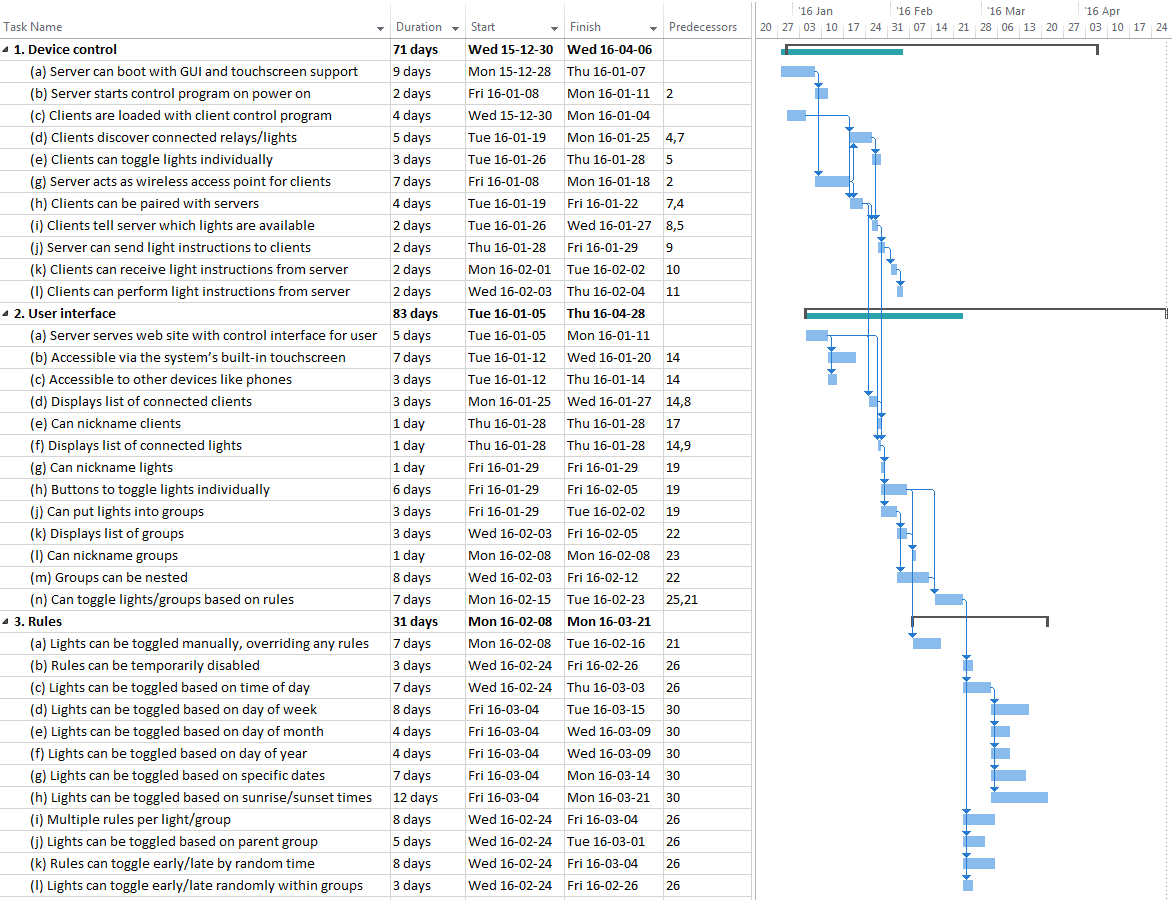
\includegraphics[width=1.0\textwidth]{ganttchart-updated.png}
\end{sidewaysfigure}
\pagebreak
